\documentclass{article}

\usepackage{geometry}

\geometry{a4paper}

%\usepackage[UTF8, heading = false, scheme = plain]{ctex}%格式

\usepackage{ctex}

%\usepackage{authblk} %添加机构 安装preprint后可用

\usepackage{graphicx} %添加图片

\usepackage{amsthm}

\usepackage{amsmath}

\renewcommand{\vec}[1]{\boldsymbol{#1}} % 生产粗体向量,而不是带箭头的向量

\usepackage{amssymb}

\usepackage{booktabs} % excel导出的大表格

\usepackage{hyperref}

\usepackage{graphicx} 

\usepackage{subfigure}
\usepackage{tikz}
\usepackage{color}
\usetikzlibrary {datavisualization.formats.functions}

\usetikzlibrary{positioning}%为了实现相对位置的设定

\usepackage{xcolor}
%\newtheorem{definition}{Definition} %英文

%\newtheorem{theorem}{Theorem}

\newtheorem{definition}{定义} %中文

\newtheorem{lemma}{引理}

\newtheorem{theorem}{定理}

%\newenvironment{proof}{{\noindent\it 证明}\quad}{\hfill □ \square□\par}

\DeclareMathOperator{\Ima}{Im}%定义新符号

\DeclareMathOperator{\Rank}{rank}%定义求秩算子

\title{cMCP方法下无关特征权重趋于零的证明}

\author{xlt}

%\affil{中国科学院} 
%需要把上面的\usepackage{authblk}取消注释

%date{}

\begin{document}

\maketitle

%\tableofcontents

%\newpage

%\listoffigures

%\newpage

\section{标识}

%\begin{figure}[ht] %htbp

%\centering

%\includegraphics[scale=0.6]{ai.png}

%\caption{this is a figure demo}

%\label{fig:label}

%\end{figure}
损失函数的形式为:
\begin{equation}\label{loss}
	Loss_{\eta}(y,\pmb{x})=P_1(W_{1,.,.}^{(\eta)})+J(W^{(\eta)})_{m}
\end{equation}
\qquad 其中$(\pmb{x},y)$是观测值,$\eta=\left\{(W_a,b_a)\right\}^{L+1}_{a=1}$是神经网络参数,$W$是权重,$P_1(\cdot)$是cMCP方法,$J(\cdot)_m$是余弦裕度交叉熵损失。并且记有关特征构成的集合为$S$,无关特征构成的集合为$S_c$。
\par 所以本文的核心是解决以下最优问题:
\begin{equation}\label{hateta}
	\begin{aligned}
	    &\hat{\eta}\in\underset{\eta \in \Theta}{\arg \min}\ P_1(W_{1,.,.}^{(\eta)})+J(W^{(\eta)})_{m}\\
	     wh&ere\ \Theta=\left\{\eta\in\mathbb{R}^q:\left\|other(\eta)\right\|_2\leq K\right \}
	\end{aligned}
\end{equation}
其中$K$为任意大于$0$的常数,并且定义:
\begin{equation}\label{other}
	\text{other}(\eta)=(b_1,\left\{(W_a,b_a)\right\}_{a=2}^{L+1})
\end{equation}
\par 定义期望损失最小的最优神经网络集合为:
\begin{equation}\label{EQ}
	EQ^*=\underset{\eta \in \Theta}{\arg \min}\ \mathbb{P}J(W^{(\eta)})
\end{equation}
其中$\mathbb{P}$是$\pmb{x}$和$y$联合分布的期望,\textcolor{red}{$\Theta$是一个足够大的集合,从而使得$\forall \eta^* \in EQ^*$的无关特征权重都为$0$}。同时对于$\forall\eta$,定义$EQ^*$中离其最近的点$\eta^{*(\eta)}$为:
\begin{equation}\label{definationofstar}
	\begin{split}
		\eta^{*(\eta)}=\left\{(W_a^{*(\eta)},b_a^{*(\eta)})\right\}_{a=1}^{L+1}\in \underset{\eta^*\in EQ^*}{\arg \min}\left\|\eta-\eta^*\right\|_2
	\end{split}
\end{equation}
\par 另有神经网络$\eta$的超额损失为:
\begin{equation}\label{excessloss}
\begin{aligned}
	\varepsilon(\eta)&=\mathbb{P}J(W^{(\eta)})_m-\mathbb{P}J(W^{*(\eta)})_m\\
	&=\mathbb{P}\left[J(W^{(\eta)}_m-J(W^{*(\eta)})_m\right]
\end{aligned}
\end{equation}
\section{证明过程}
\subsection{第一阶段}
根据$\hat{\eta}$的定义可知,其满足对于$\forall \eta \in \Theta$,有:
\begin{equation}
	\begin{aligned}
		Loss_{\hat{\eta}}(y,\pmb{x})&\leq Loss_{\eta^{*(\hat{\eta})}}(y,\pmb{x})\\
		\sum_{j=1}^p P_1(W_{1,.,j}^{(\hat{\eta})})+\mathbb{P}_nJ(W^{(\hat{\eta})})_m&\leq\sum_{j=1}^p P_1(W_{1,.,j}^{*(\hat{\eta})})+\mathbb{P}_nJ(W^{*(\hat{\eta})})_m
	\end{aligned}
\end{equation}
由于$\forall \eta^* \in EQ^*$对于无关特征的权重都为$0$,则$\forall j\in S_c,P_1(W_{1,.,j}^{*(\hat{\eta})})=0$所以有:
\begin{equation}
	\begin{aligned}
		\sum_{j=1}^p P_1(W_{1,.,j}^{*(\hat{\eta})})&=\sum_{j\in S} P_1(W_{1,.,j}^{*(\hat{\eta})})+\sum_{j\in S_c} P_1(W_{1,.,j}^{*(\hat{\eta})})\\
		&=\sum_{j\in S} P_1(W_{1,.,j}^{*(\hat{\eta})})
	\end{aligned}
\end{equation}
带回$(5)$式有:
\begin{equation}
	\begin{aligned}
		\sum_{j=1}^p P_1(W_{1,.,j}^{(\hat{\eta})})+\mathbb{P}_nJ(W^{(\hat{\eta})})_m\leq&\sum_{j \in S} P_1(W_{1,.,j}^{*(\hat{\eta})})+\mathbb{P}_nJ(W^{*(\hat{\eta})})_m\\
		\mathbb{P}J(W^{(\hat{\eta})})_m-\mathbb{P}J(W^{*(\hat{\eta})})_m+\sum^p_{j=1}P_1(W_{1,.,j}^{(\hat{\eta})})\leq&|(\mathbb{P}_n-\mathbb{P})(J(W^{*(\hat{\eta})})_m-J(W^{(\hat{\eta})})_m)|\\&+\sum_{j\in S} P_1(W_{1,.,j}^{*(\hat{\eta})})\\
	\end{aligned}
\end{equation}
最终可得:
\begin{equation}\label{firstresult}
	\varepsilon(\hat{\eta})+\sum^p_{j=1}P_1(W_{1,.,j}^{(\hat{\eta})})\leq|(\mathbb{P}_n-\mathbb{P})(J(W^{*(\hat{\eta})})_m-J(W^{(\hat{\eta})})_m)|+\sum_{j\in S} P_1(W_{1,.,j}^{*(\hat{\eta})})\\
\end{equation}
\subsection{第二阶段}
\par \textcolor{red}{现给定$\forall\tilde{\lambda}>0$,$T\geq1$有集合:
\begin{equation}
	\begin{split}
		&\tau_{\tilde{\lambda},T}=\\&\left\{(\pmb{x_i},y_i)^n_{i=1}:\underset{\eta \in \Theta}{\sup}\frac{|(\mathbb{P}_n-\mathbb{P})(J(W^{*(\hat{\eta})})_m-J(W^{(\hat{\eta})})_m)|}{\tilde{\lambda}\vee(\left\|\text{other}(\hat{\eta})-\text{other}(\eta^{*(\hat{\eta})})\right\|_2+\sum_{j=1}^pP_1(W_{1,.,j}^{(\hat{\eta})}-W_{1,.,j}^{*(\hat{\eta})}))}\leq T\tilde{\lambda}\right\}
	\end{split}
\end{equation}
}上式中引入新运算符号“$\vee$”:$a\vee b=max(a,b)$。故式(\ref*{firstresult})可以变化为:
\begin{equation}\label{imp}
	\begin{split}
		\varepsilon(\hat{\eta})+\sum^p_{j=1}P_1(W_{1,.,j}^{(\hat{\eta})})\leq &T\tilde{\lambda}(\tilde{\lambda}\vee(\left\|\text{other}(\hat{\eta})-\text{other}(\eta^{*(\hat{\eta})})\right\|_2\\&+\sum_{j=1}^pP_1(W_{1,.,j}^{(\hat{\eta})}-W_{1,.,j}^{*(\hat{\eta})})))+\sum_{j\in S} P_1(W_{1,.,j}^{*(\hat{\eta})})
	\end{split}
\end{equation}
\par 故现在需要考虑两种情况:
\begin{itemize}
	\item [1)]$\tilde{\lambda}\geq(\left\|\text{other}(\hat{\eta})-\text{other}(\eta^{*(\hat{\eta}})\right\|_2+\sum_{j=1}^pP_1(W_{1,.,j}^{(\hat{\eta})}-W_{1,.,j}^{*(\hat{\eta})})))$:
	\par 故此时式(\ref*{imp})可以变换为:
	\begin{equation}
		\begin{split}\label{type1}
			\varepsilon(\hat{\eta})+\sum^p_{j=1}P_1(W_{1,.,j}^{(\hat{\eta})})&\leq T\tilde{\lambda}\cdot\tilde{\lambda}+\sum_{j\in S} P_1(W_{1,.,j}^{*(\hat{\eta})})\\
			\varepsilon(\hat{\eta})+\sum_{j\in S_c}P_1(W_{1,.,j}^{(\hat{\eta})})&\leq T\tilde{\lambda}\cdot\tilde{\lambda}+\sum_{j\in S} (P_1(W_{1,.,j}^{*(\hat{\eta})})-P_1(W_{1,.,j}^{(\hat{\eta})}))
		\end{split}
	\end{equation}
	\textcolor{red}{由于$P_1(\cdot)$函数的基本形式保证了其定义域中的$\forall x_1,x_2$有:
	\begin{equation}\label{inequilty}
		P_1(x_1+x_2)\leq P_1(x_1)+P_1(x_2)
	\end{equation}}
	且在该情况下$\tilde{\lambda}$满足$\tilde{\lambda}\geq\sum_{j\in S}P_1(W_{1,.,j}^{*(\hat{\eta})}-W_{1,.,j}^{(\hat{\eta})}))$所以式(\ref*{type1})可以变换为:
	\begin{equation}
		\begin{split}
		\varepsilon(\hat{\eta})+\sum_{j\in S_c}P_1(W_{1,.,j}^{(\hat{\eta})})&\leq T\tilde{\lambda}^2+\tilde{\lambda}\\
		    \sum_{j\in S_c}P_1(W_{1,.,j}^{(\hat{\eta})})&\leq T\tilde{\lambda}^2+\tilde{\lambda}
		\end{split}
	\end{equation}
	\item [2)]$\tilde{\lambda}<(\left\|\text{other}(\hat{\eta})-\text{other}(\eta^{*(\hat{\eta}})\right\|_2+\sum_{j=1}^pP_1(W_{1,.,j}^{(\hat{\eta})}-W_{1,.,j}^{*(\hat{\eta})})))$:
	\par 故此时式(\ref*{imp})可以变换为:
	\begin{equation}
		\begin{split}\label{type2}
			\varepsilon(\hat{\eta})+\sum^p_{j=1}P_1(W_{1,.,j}^{(\hat{\eta})})\leq &T\tilde{\lambda}(\left\|\text{other}(\hat{\eta})-\text{other}(\eta^{*(\hat{\eta})})\right\|_2+\sum_{j=1}^pP_1(W_{1,.,j}^{(\hat{\eta})}-W_{1,.,j}^{*(\hat{\eta})})))\\&+\sum_{j\in S}P_1(W_{1,.,j}^{*(\hat{\eta})})
		\end{split}
	\end{equation}
	由于$\forall j\in S_c,P_1(W_{1,.,j}^{*(\hat{\eta})})=0$和式(\ref*{inequilty}),有:
	\begin{equation}\label{pretype2result}
		\begin{split}
		    \varepsilon(\hat{\eta})+(1-T\tilde{\lambda})\sum_{j\in S_c}P_1(W_{1,.,j}^{(\hat{\eta})})\leq &T\tilde{\lambda}\left\|\text{other}(\hat{\eta})-\text{other}(\eta^{*(\hat{\eta})})\right\|_2+\\&(1+T\tilde{\lambda})\sum_{j\in S}P_1(W_{1,.,j}^{(\hat{\eta})}-W_{1,.,j}^{*(\hat{\eta})}))\\
		\end{split}
	\end{equation}
	将式(\ref*{pretype2result})化简,并将常数项移至右侧,可得:
	\begin{equation}\label{type2result}
		\begin{split}
			\sum_{j\in S_c}P_1(W_{1,.,j}^{(\hat{\eta})})&\leq \frac{T\tilde{\lambda}}{(1-T\tilde{\lambda})}\left\|\text{other}(\hat{\eta})-\text{other}(\eta^{*(\hat{\eta})})\right\|_2\\&+\frac{(1+T\tilde{\lambda})}{(1-T\tilde{\lambda})}\sum_{j\in S}P_1(W_{1,.,j}^{(\hat{\eta})}-W_{1,.,j}^{*(\hat{\eta})}))	
		\end{split}
	\end{equation}
\end{itemize}
\par 在集合$\tau_{T,\tilde{\lambda}}$下,综合考虑两种情况可知无关特征在cMCP方法中的损失一定满足式(\ref*{type2result})。
\subsection{第三阶段}
现讨论无关权重在损失函数中的损失与其权重大小之间的关系。
\par 根据$\rho(\cdot)$函数的图(图1)可得
\begin{figure}
\begin{center}
	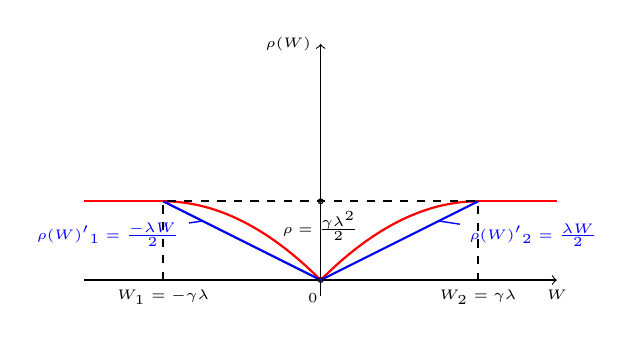
\begin{tikzpicture}
		\draw[->](-3,0)--(3,0)node[below,font=\tiny]{$W$};
    \draw[->](0,-0.2)--(0,3)node[left,font=\tiny]{$\rho(W)$};
    \draw[color=red, thick,smooth,domain=0:2]plot(\x,\x-\x*\x/4);
	\draw[color=red, thick,smooth,domain=2:3]plot(\x,1);
	\draw[color=red, thick,smooth,domain=-2:0]plot(\x,-\x-\x*\x/4);
	\draw[color=red, thick,smooth,domain=-3:-2]plot(\x,1);
	\draw[color=blue, thick,smooth,domain=0:2]plot(\x,0.5*\x) ;
	\path[color=blue] (2.7,0.3) node(r2)[right,above,font=\tiny]{$\rho(W){'}_2=\frac{\lambda W}{2}$};
	\path[color=blue] (-2.7,0.3) node(r1)[right,above,font=\tiny]{$\rho(W){'}_1=\frac{-\lambda W}{2}$};
	\path[color=black] (-0.1,-0.05) node(r3)[left,below,font=\tiny]{$0$};
	\draw[color=blue, thick,smooth,domain=0:-2]plot(\x,-0.5*\x) ;
	\draw[line width=0.5pt,color=blue] (r1)--(-1.5,0.75); 
	\draw[line width=0.5pt,color=blue] (r2)--(1.5,0.75); 
    \draw[color=black,smooth]circle(0.03);
	\draw[color=black,smooth](0,1)circle(0.03);
	\draw [thick, dashed,font=\tiny]  (-2,0) node [below] {$W_1=-\gamma\lambda$}--(-2,1)--(0,1) node [left,below] {$\rho=\frac{\gamma \lambda^2}{2}$} -- (2,1)
       -- (2,0) node [below] {$W_2=\gamma\lambda$};
	\end{tikzpicture}
	\end{center}
	\caption{$\rho(W)$图像}
    \end{figure}
	\label{rhofig}
当该函数的自变量$W$的绝对值非常小时,其满足:
\begin{equation}
	\rho(W)>\frac{1}{2}\lambda |W|
\end{equation}
\par 同时根据$P_1(\cdot)$的损失函数的泰勒展开具有下列形式:
\begin{equation}
	\begin{split}
		P_1(W_{1,.,.}^{(\hat{\eta})})&=\sum_{j=1}^p\rho_1(\sum_r^{K(1)}\rho_2(W_{1,r,j}^{(\hat{\eta})};\lambda_2,\gamma_2);\lambda_1,\gamma_1)\\
		&\geq \sum_{j=1}^p\rho_1(\frac{1}{2}\lambda_2\sum_r^{K(1)}|W_{1,r,j}^{(\hat{\eta})}|;\lambda_1,\gamma_1)\\
		&\geq \frac{1}{4}\lambda_1\lambda_2\sum_{j=1}^p\sum_r^{K(1)}|W_{1,r,j}^{(\hat{\eta})}|\\
		&=\frac{1}{4}\lambda_1\lambda_2\left\|W_{1,.,.}^{(\hat{\eta})}\right\|_1
	\end{split}
\end{equation}
所以无关特征的损失函数可以表示为:
\begin{equation}
	P_1(W_{1,.,S_c}^{(\hat{\eta})})\geq \frac{1}{4}\lambda_1\lambda_2\left\|W_{1,.,S_c}^{(\hat{\eta})}\right\|_1
\end{equation}
\par 根据式(\ref*{type2result})可得:
\begin{equation}
	\begin{split}
		\frac{1}{4}\lambda_1\lambda_2\left\|W_{1,.,S_c}^{(\hat{\eta})}\right\|_1\leq&\frac{T\tilde{\lambda}}{(1-T\tilde{\lambda})}\left\|\text{other}(\hat{\eta})-\text{other}(\eta^{*(\hat{\eta})})\right\|_2\\&+\frac{(1+T\tilde{\lambda})}{(1-T\tilde{\lambda})}\sum_{j\in S}P_1(W_{1,.,j}^{(\hat{\eta})}-W_{1,.,j}^{*(\hat{\eta})}))\\
	\end{split}
\end{equation}
最终可得到无关权重的向量$S_c$在最优网络的输入层的权重$W_{1,.,S_c}^{(\hat{\eta})}$满足:
\begin{equation}\label{quanzhongsc}
	\begin{split}
		\left\|W_{1,.,S_c}^{(\hat{\eta})}\right\|_1\leq &\frac{4T\tilde{\lambda}}{(1-T\tilde{\lambda})\lambda_1\lambda_2}\left\|\text{other}(\hat{\eta})-\text{other}(\eta^{*(\hat{\eta})})\right\|_2\\&+\frac{4(1+T\tilde{\lambda})}{(1-T\tilde{\lambda})\lambda_1\lambda_2}\sum_{j\in S}P_1(W_{1,.,j}^{(\hat{\eta})}-W_{1,.,j}^{*(\hat{\eta})}))
	\end{split}
\end{equation}
\textcolor{red}{其中的参数$T\le1$和$\tilde{\lambda}>0$是任意给定的,参数$\lambda_1$和$\lambda_2$是损失函数决定的,所以式(\ref*{quanzhongsc})右侧的$\frac{4T\tilde{\lambda}}{(1-T\tilde{\lambda})\lambda_1\lambda_2}$和$\frac{4(1+T\tilde{\lambda})}{(1-T\tilde{\lambda})\lambda_1\lambda_2}$可以看成常数。}
\subsection{第四部分}
由于式(\ref*{quanzhongsc})的右侧部分为两个常数与函数或者函数的范数相乘的形式,所以对其中函数或函数的范数进行讨论。
\par 先讨论右边的第一部分,根据式(\ref*{other})中$other(\cdot)$的定义可知:
\begin{equation}\label{2other}
	\begin{split}
		\left\|\text{other}(\hat{\eta})-\text{other}(\eta^{*(\hat{\eta})})\right\|_2&=\left\|(b_1^{(\hat{\eta})},\left\{(W_a^{(\hat{\eta})},b_a^{(\hat{\eta})})\right\}_{a=2}^{L+1})-(b_1^{*(\hat{\eta})},\left\{(W_a^{*(\hat{\eta})},b_a^{*(\hat{\eta})})\right\}_{a=2}^{L+1})\right\|_2\\
		&=\left\|(b_1^{(\hat{\eta})}-b_1^{*(\hat{\eta})}),\left\{(W_a^{(\hat{\eta})}-W_a^{*(\hat{\eta})}),(b_a^{(\hat{\eta})}-b_a^{*(\hat{\eta})})\right\}_{a=2}^{L+1}\right\|_2\\
		&=\left\|(W_a^{(\hat{\eta})}-W_a^{*(\hat{\eta})})_{a=2}^{L+1},(b_a^{(\hat{\eta})}-b_a^{*(\hat{\eta})})_{a=1}^{L+1}\right\|_2\\
		&\leq\sum_{a=1}^{L+1}\left\|b_a^{(\hat{\eta})}-b_a^{*(\hat{\eta})}\right\|_2+\sum_{a=2}^{L+1}\left\|W_a^{(\hat{\eta})}-W_a^{*(\hat{\eta})}\right\|_2
	\end{split}
\end{equation}
\par 根据切比雪夫不等式可知,对于$\forall\varepsilon>0$有:
\begin{equation}\label{chiinequity}
	\begin{split}
		P(\left\|b_a^{(\hat{\eta})}-b_a^{*(\hat{\eta})}\right\|_2\ge\varepsilon)\leq\frac{\left\|b_a^{(\hat{\eta})}-b_a^{*(\hat{\eta})}\right\|_2^2}{\varepsilon}
	\end{split}
\end{equation}
再根据$\eta^{*(\hat{\eta})}$的定义可知,其是$EQ^*$中离$\hat{\eta}$最近的点,所以有:$\left\|b_a^{(\hat{\eta})}-b_a^{*(\hat{\eta})}\right\|_2^2\to 0$,同时由于$\varepsilon$是一个任意常数,所以式(\ref*{chiinequity})有集合:
\begin{equation}
	\begin{split}
		\lim P(\left\|b_a^{(\hat{\eta})}-b_a^{*(\hat{\eta})}\right\|_2\ge\varepsilon)=0
	\end{split}
\end{equation}
故有:$\left\|b_a^{(\hat{\eta})}-b_a^{*(\hat{\eta})}\right\|_2\xrightarrow{P}0$。同样地,可以证明:$\left\|W_a^{(\hat{\eta})}-W_a^{*(\hat{\eta})}\right\|_2\xrightarrow{P}0$,所以这两部分求和结果的加和同样满足,所以可以得到:$\left\|\text{other}(\eta)-\text{other}(\eta^{*(\eta)})\right\|_2\xrightarrow{P}0$。
\par 再讨论右边的第二部分。根据$P_1(\cdot)$函数所具有的对称性,对于$\forall j\in S$有:
\begin{equation}
	\begin{split}
		P_1(W_{1,.,j}^{(\hat{\eta})}-W_{1,.,j}^{*(\hat{\eta})}))&=P_1(|W_{1,.,j}^{(\hat{\eta})}-W_{1,.,j}^{*(\hat{\eta})})|)
	\end{split}
\end{equation}
\par 同样地,根据$\eta^{*(\hat{\eta})}$的定义以及切比雪夫不等式可知$|W_{1,.,j}^{(\hat{\eta})}-W_{1,.,j}^{*(\hat{\eta})})|\xrightarrow{P}0$。
\par 根据依概率收敛的引理:若$f(\cdot )$在$c$处连续,且$Yn\xrightarrow{P}c$,则有:$f(Yn)\xrightarrow{P}f(c)$。由于$P(\cdot)$在其定义域上都连续,且$P_1(0)=0$所以有:
\begin{equation}
	\begin{split}
		P_1(|W_{1,.,j}^{(\hat{\eta})}-W_{1,.,j}^{*(\hat{\eta})})|)\xrightarrow{P}P_1(0)=0
	\end{split}
\end{equation}
则其求和的结果$\sum_{j\in S}P_1(W_{1,.,j}^{(\hat{\eta})}-W_{1,.,j}^{*(\hat{\eta})}))$也同样依概率收敛于0。
\par 至此,式(\ref*{quanzhongsc})两部分都依概率收敛于0得证,又$\left\|W_{1,.,S_c}^{(\hat{\eta})}\right\|_1\ge0$,所以根据迫敛性有:
\begin{equation}
	\begin{split}
		\left\|W_{1,.,S_c}^{(\hat{\eta})}\right\|_1\longrightarrow 0
	\end{split}
\end{equation}
\textcolor{red}{所以,训练得到的最优网络结构$\hat{\eta}$满足所有无关特征的第一层权重收敛于0,所以在其在后续隐藏层中的权重也收敛于0.因此,cMCP方法下训练得到的网络结构使得无关特征权重趋于0得证。}
\end{document}

